\documentclass[arhiv]{../izpit}
\usepackage{fouriernc}
\usepackage{tikz}
\usepackage{censor}
\usepackage{paralist}
\usepackage{listings}
\usepackage{changepage}
\usepackage{paralist}
\usepackage{amssymb}

\begin{document}

\izpit{Programiranje I: 1.\ izpit}{2.\ svečana leta Gospodovega 2015}{
  Čas reševanja je 150 minut.
  Doseženih 100 točk šteje za maksimalno oceno.
  Veliko uspeha!
}

%%%%%%%%%%%%%%%%%%%%%%%%%%%%%%%%%%%%%%%%%%%%%%%%%%%%%%%%%%%%%%%%%%%%%%
\naloga[Skakačev sprehod, 30 točk]

Dana je šahovnica velikosti $n \times n$. Polje v $r$-ti vrstici in $c$-tem stolpcu označimo z $(r, c)$, $1 \leq r, c \leq n$. Zaporedje polj
$$
(r_1, c_1), (r_2, c_2), (r_3, c_3), \ldots, (r_{k}, c_{k})
$$
opisuje veljaven skakačev sprehod, če velja:
\begin{compactenum}
\renewcommand{\labelenumi}{\alph{enumi})}
\item $|r_i - r_{i+1}| = 2 \land |c_i - c_{i+1}| = 1$ ali $|r_i - r_{i+1}| = 1 \land |c_i - c_{i+1}| = 2$ za vse $1 \leq i < k$ (tj. skakač dela premike v obliki črke L);
\item vsako polje šahovnice obišče natanko enkrat.
\end{compactenum}

\vspace{\baselineskip}

\noindent V \emph{Mathematici} sestavite funkcijo \texttt{veljavenSprehod[sprehod\_, n\_]}, ki kot argumenta dobi:
\begin{compactitem}
\item seznam, ki opisuje sprehod skakača, in
\item velikost šahovnice.
\end{compactitem}
Funkcija naj vrne \texttt{True}, če je sprehod veljaven, in \texttt{False} sicer. Primer:
%
\begin{verbatim}
In[1]:= sprehod = {{1, 2}, {2, 4}, {4, 3}, {3, 1}, {2, 3}, {4, 4}};
In[2]:= veljavenSprehod[sprehod, 4]
Out[2]= False
\end{verbatim}

\noindent Nasvet 1: Najprej sestavite dve pomožni funkciji. Prva naj preveri pogoj a), druga pa pogoj b).

\vspace{0.5\baselineskip}
\noindent Nasvet 2: Za katere pare polj $(r, c)$ in $(\tilde{r}, \tilde{c})$ velja $|r - \tilde{r}| \cdot |c - \tilde{c}| = 2$?

\vspace{0.5\baselineskip}
\noindent Nasvet 3: Kaj vrne \texttt{Sort[\{\{1, 2\}, \{2, 4\}, \{4, 3\}, \{3, 1\}, \{2, 3\}, \{4, 4\}\}]}?

%%%%%%%%%%%%%%%%%%%%%%%%%%%%%%%%%%%%%%%%%%%%%%%%%%%%%%%%%%%%%%%%%%%%%%
\naloga[Möbiusova lestev, 30 točk]

V \emph{Mathematici} sestavite funkcijo \texttt{lestev[n\_]}, ki nariše Möbiusovo lestev reda $n$. Slika grafa naj ima vozlišča ekvidistančno razporejena na dveh krožnicah (s polmeroma 1 in 2); na vsaki krožnici naj bo $n$ vozlišč. Vsako ``notranje'' vozlišče je povezano z ustreznim ``zunanjim'' vozliščem. Povezave so tudi med zaporednimi vozlišči na notranji oz.\ zunanji krožnici, razen na enem mestu, kjer se povezavi ``prekrižata'', kakor lahko vidite na primerih:

\begin{center}
\begin{tabular}{c@{\hspace{1.5cm}}c@{\hspace{1.5cm}}c}
 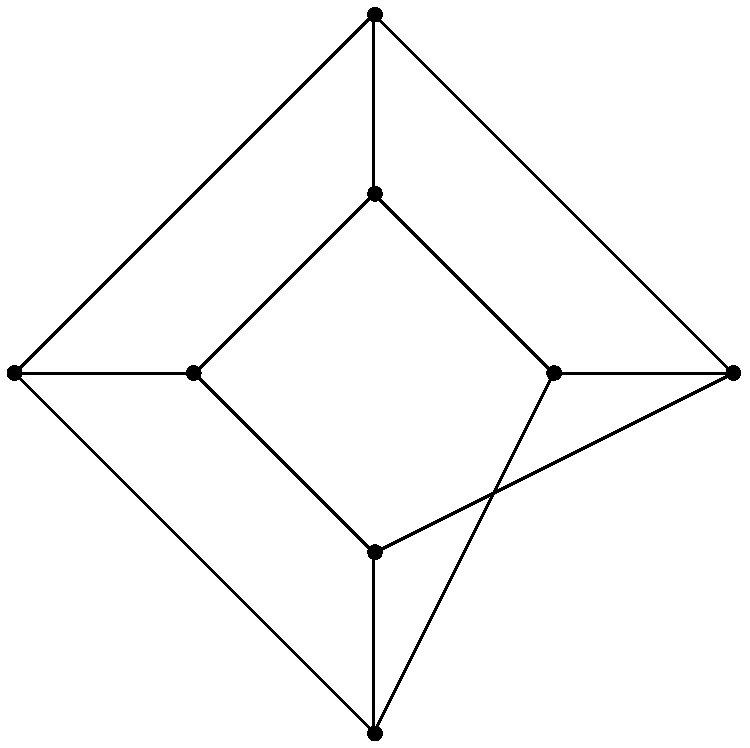
\includegraphics[width=4cm]{lestev4.pdf}&
 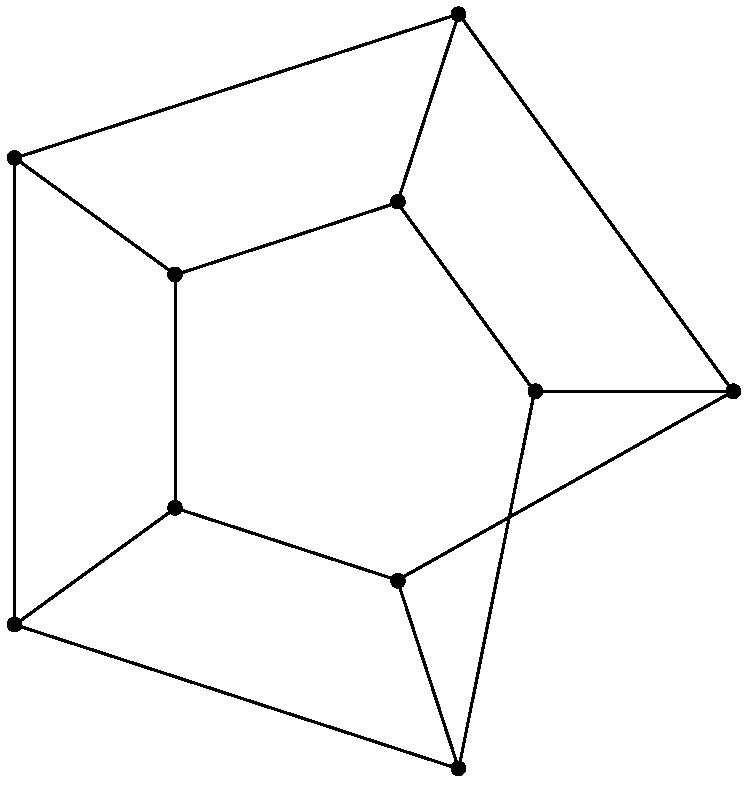
\includegraphics[width=4cm]{lestev5.pdf}&
 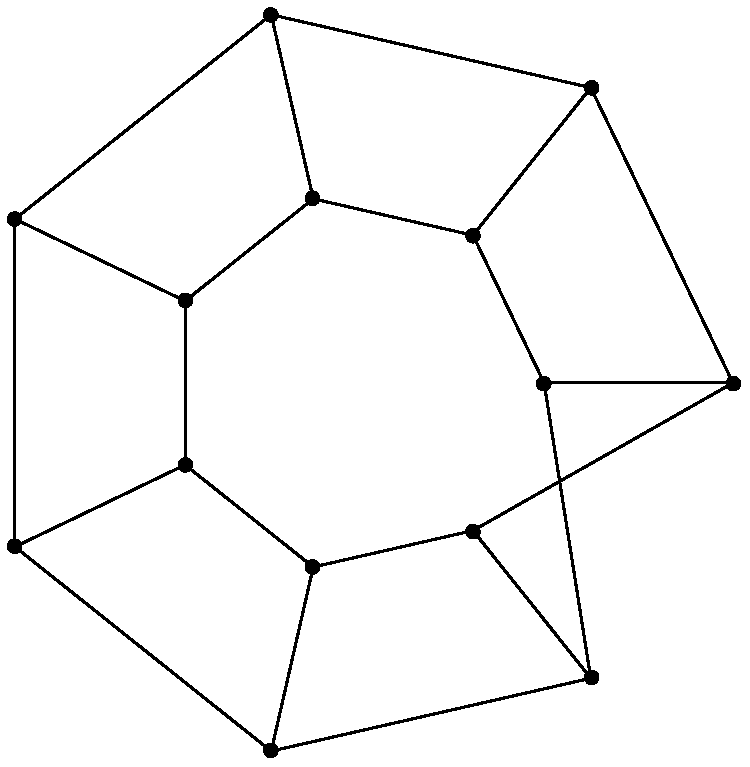
\includegraphics[width=4cm]{lestev7.pdf}\\
  \texttt{lestev[4]} &
  \texttt{lestev[5]} &
  \texttt{lestev[7]}
\end{tabular}
\end{center}

Še formalna definicija Möbiusove lestve $M_n$:
\begin{eqnarray*}
V(M_n) & = & \big\{(i, j) \mid 0 \leq i < n, 0 \leq j \leq 1 \big\} \\
E(M_n) & = & \big\{\{(i, 0), (i, 1)\} \mid 0 \leq i < n \big\} \cup \big\{\{(i, 0), (i+1, 0)\} \mid 0 \leq i < n-1 \big\} \cup \\
 & & \big\{\{(i, 1), (i+1, 1)\} \mid 0 \leq i < n-1 \big\} \cup \big\{ \{(0,0), (n-1,1)\}, \{(0,1), (n-1,0)\} \big\}
\end{eqnarray*}

%%%%%%%%%%%%%%%%%%%%%%%%%%%%%%%%%%%%%%%%%%%%%%%%%%%%%%%%%%%%%%%%%%%%%%
\naloga[Zasnežena cesta, 10 + 10 + 10 točk]

% \begin{adjustwidth}{3em}{3em}
% \emph{Zima bleda starka je snega nasula,\\
% drevju bele čevlje zopet je obula,\\
% z belo je preprogo travnik pogrnila,\\
% a veseli potok ves leden molči.} --- Čuki, Sankaška polka
% \end{adjustwidth}
% \vspace{0.5\baselineskip}

\noindent Izdelali bomo razred \texttt{Cesta}, ki bo v pomoč snežni službi, ki skrbi za čiš\-čenje zelo dolge ceste. Cesta je razdeljena na kilometrske odseke, ki so oštevilčeni od 1 do $n$. Predstavimo jo lahko s drevesom, kot ga vidite na sliki (primer za $n = 7$):
$$
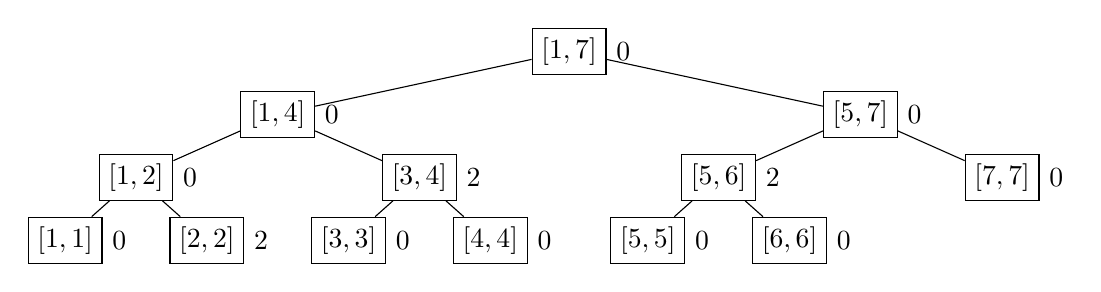
\begin{tikzpicture}[level distance=0.8cm,
    level 1/.style={sibling distance=7.4cm},
    level 2/.style={sibling distance=3.6cm},
    level 3/.style={sibling distance=1.8cm}
    ]
    \node[rectangle, draw, label=0:0] (d) {$[1, 7]$}
      child {node[rectangle, draw, label=0:0] {$[1, 4]$}
        child {node[rectangle, draw, label=0:0] {$[1, 2]$}
          child {node[rectangle, draw, label=0:0] {$[1, 1]$}}
          child {node[rectangle, draw, label=0:2] {$[2, 2]$}}
        }
        child {node[rectangle, draw, label=0:2] {$[3, 4]$}
          child {node[rectangle, draw, label=0:0] {$[3, 3]$}}
          child {node[rectangle, draw, label=0:0] {$[4, 4]$}}
        }
      }
      child {node[rectangle, draw, label=0:0] {$[5, 7]$}
        child {node[rectangle, draw, label=0:2] {$[5, 6]$}
          child {node[rectangle, draw, label=0:0] {$[5, 5]$}}
          child {node[rectangle, draw, label=0:0] {$[6, 6]$}}
        }
        child {node[rectangle, draw, label=0:0] {$[7, 7]$}}
      };
  \end{tikzpicture}
$$
Razred \texttt{Cesta} (ki je nekakšno dvojiško drevo) je že delno implementiran. Vsako vozlišče predstav\-lja nek interval odsekov in ima atributa \texttt{zacetek} in \texttt{konec}. Koren predstavlja celotno cesto in ima $\texttt{zacetek} = 1$ in $\texttt{konec} = n$. Če je $\texttt{zacetek} \neq \texttt{konec}$, ima vozlišče še atributa \texttt{levo} in \texttt{desno}, ki predstavljata levi in desni podinterval. Vsak podinterval pokriva polovico odsekov (oz. je levi za 1 daljši, če število odsekov ni sodo).

Poleg tega ima vsako vozlišče še atribut \texttt{sneg}, ki predstavlja količino snega na tem intervalu (števila, ki so zapisana desno od vozlišč na zgornji sliki). Če bi bila cesta v celoti očiščena, bi povsod imeli vrednost $0$. Ker je na $[2, 6]$ zapadlo 2 cm snega, imamo ponekod vrednost 2. Atribut \texttt{sneg} smo povečali samo pri tistih vozliščih, za katere velja, da:
\begin{compactenum}
\renewcommand{\labelenumi}{\alph{enumi})}
\item so v celoti vsebovana v $[2, 6]$ in
\item njihov oče ni v celoti vsebovan v $[2, 6]$.
\end{compactenum}
Tako smo atributu \texttt{sneg} vozlišča $[3, 4]$ prišteli 2, saj $[3, 4] \subseteq [2, 6]$ in $\mathrm{oče}([3, 4]) = [1, 4] \nsubseteq [2, 6]$. Atributu \texttt{sneg} vozlišča $[5, 5]$ pa nismo prišteli nič, saj $\mathrm{oče}([5, 5]) = [5, 6] \subseteq [2, 6]$.

\podnaloga[10 točk]
Sestavite metodo \texttt{zasnezi(self, a, b, k)}, ki strukturo \texttt{Cesta} ustrezno spremeni, če na odsekih $[a, b]$ zapade $k$ centimetrov snega. Primer (če \texttt{c} ustreza zgornji sliki):
%
\begin{verbatim}
>>> c.zasnezi(5, 7, 3)
>>> c.zasnezi(1, 3, 1)
>>> c.seznam()
[1, 3, 3, 2, 5, 5, 3]
\end{verbatim}
Novo stanje:
$$
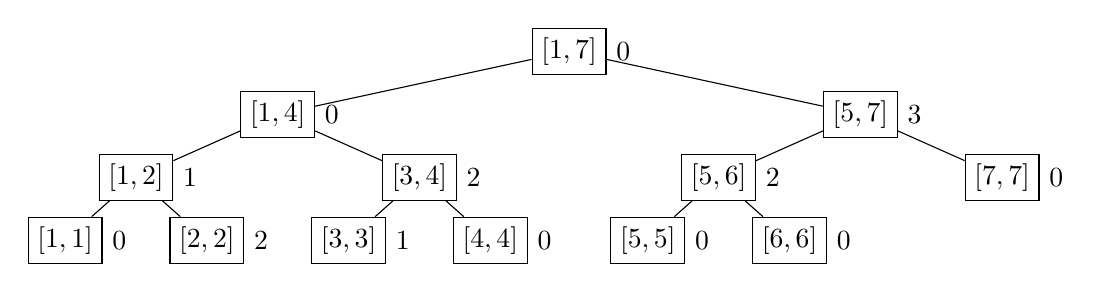
\begin{tikzpicture}[level distance=0.8cm,
    level 1/.style={sibling distance=7.4cm},
    level 2/.style={sibling distance=3.6cm},
    level 3/.style={sibling distance=1.8cm}
    ]
    \node[rectangle, draw, label=0:0] (d) {$[1, 7]$}
      child {node[rectangle, draw, label=0:0] {$[1, 4]$}
        child {node[rectangle, draw, label=0:1] {$[1, 2]$}
          child {node[rectangle, draw, label=0:0] {$[1, 1]$}}
          child {node[rectangle, draw, label=0:2] {$[2, 2]$}}
        }
        child {node[rectangle, draw, label=0:2] {$[3, 4]$}
          child {node[rectangle, draw, label=0:1] {$[3, 3]$}}
          child {node[rectangle, draw, label=0:0] {$[4, 4]$}}
        }
      }
      child {node[rectangle, draw, label=0:3] {$[5, 7]$}
        child {node[rectangle, draw, label=0:2] {$[5, 6]$}
          child {node[rectangle, draw, label=0:0] {$[5, 5]$}}
          child {node[rectangle, draw, label=0:0] {$[6, 6]$}}
        }
        child {node[rectangle, draw, label=0:0] {$[7, 7]$}}
      };
  \end{tikzpicture}
$$

\podnaloga[10 točk]
Napišite metodo \texttt{kolicina(self, t)}, ki vrne količino snega na $t$-tem odseku ceste. Primer (če \texttt{c} ustreza zadnjemu stanju ceste):
%
\begin{verbatim}
>>> c.kolicina(6)
5
\end{verbatim}

\podnaloga[10 točk]
Sestavite metodo \texttt{ocisti(self, t)}, ki strukturo \texttt{Cesta} ustrezno spremeni, če plug očisti ves sneg s $t$-tega odseka ceste. Primer (če \texttt{c} ustreza zadnjemu stanju ceste):
%
\begin{verbatim}
>>> c.ocisti(6)
>>> c.seznam()
[1, 3, 3, 2, 5, 0, 3]
\end{verbatim}

%%%%%%%%%%%%%%%%%%%%%%%%%%%%%%%%%%%%%%%%%%%%%%%%%%%%%%%%%%%%%%%%%%%%%%
\naloga[Izpitno obdobje, 15 + 15 točk]
Prihaja izpitno obdobje in študentje so sklenili, da bodo rešili vse stare izpitne naloge pri vseh predmetih.
Organizirali so se in si razdelili delo. Seznam $p = [p_1, p_2, \ldots, p_n]$ predstavlja število nalog pri vsakem od $n$ predmetov. V letniku je $d$
dobrih študentov in $s$ slabih študentov. Dober študent je sposoben rešit $m$ nalog na dan, pod pogojem, da \emph{so
vse naloge iz istega predmeta}. Slabi študentje lahko rešijo le 1 nalogo na dan.

Vincenc se je vprašal, ali so sposobni rešiti vse naloge v $k$ dneh. Razmišljal je takole: 
Na voljo imamo $dk$ ``dobrih'' človek-dni in $sk$ ``slabih'' človek-dni. Dobro je, če pri vsakem predmetu naredimo paketke po $m$ nalog in jih razdelimo dobrim študentom. Tako lahko naredimo
$$
\delta = \sum_{i=1}^{n} \left\lfloor \frac{p_i}{m} \right\rfloor 
$$
takšnih paketkov, pri čemer nam ostane še
$$
p' = [p_1 \bmod m, p_2 \bmod m, \ldots, p_n \bmod m]
$$
nalog pri vsakem predmetu.
\begin{itemize}
\item
Če je $dk < \delta$, ni dovolj dobrih študentov, da bi rešili vse paketke, zato jih rešijo le $dk$ in ostane še 
$$\sigma = m(\delta - dk) +  \sum_{i=1}^{n} p_i \bmod m $$
nalog, ki jih morajo rešiti slabi študentje. Naloge je možno rešiti v danem času, če je $\sigma \leq sk$.
\item
Če pa je $dk \geq \delta$, lahko dobri študentje poskrbijo za vse paketke in ostane še
$$
\delta' = dk - \delta
$$
dobrih človek-dni. Seznam $p'$ smemo brez škode urediti nenaraščajoče (predmete lahko drugače oštevilčimo, pa se zaradi tega problem nič ne spremeni). Preostale naloge pri predmetih $1, 2, \ldots, \delta'$ lahko razdelimo med dobre študente. Slabim študentom ostane še
$$
\sigma' = \sum_{i=\delta'+1}^{n} p_i \bmod m
$$
nalog. Naloge je možno rešiti v danem času, če je $\sigma' \leq sk$.
\end{itemize}

\podnaloga[15 točk]
Sestavite funkcijo \texttt{mozno\_resiti(p, s, d, m, k)}, ki kot argumente dobi:
\begin{compactitem}
\item \texttt{p} -- seznam s številom nalog pri posameznih predmetih;
\item \texttt{s} -- število slabih študentov;
\item \texttt{d} -- število dobrih študentov;
\item \texttt{m} -- število nalog, ki so jih sposobni rešiti dobri študentje v enem dnevu;
\item \texttt{k} -- število dni, ki jih imajo študentje na voljo za reševanje nalog.
\end{compactitem}
Funkcija naj vrne \texttt{True}, če lahko študentje rešijo vse naloge v danem času, in \texttt{False} sicer. Postopajte tako, kot predlaga Vincenc.

%\podnaloga[20 točk]
%Kakšna je časovna zahtevnost algoritma iz prejšnje točke? Utemeljite.

\podnaloga[15 točk]
Napišite funkcijo \texttt{koliko\_dni(p, s, d, m)}, ki na učinkovit način izračuna najmanjše število dni, ki jih potrebujejo študentje, da rešijo vse naloge. 
\emph{Nasveti:}
\begin{compactitem}
\item Kličite funkcijo \texttt{mozno\_resiti} iz prejšnje podnaloge (tj.\ uporabljajte jo kot črno škatlo).
\item Študentje lahko naloge zagotovo rešijo v $$\left\lceil \frac{\sum_{i=1}^{n} p_i }{d + s} \right\rceil$$ dnevih (če bi se organizirali tako, da bi vsak rešil po 1 nalogo na dan).
\end{compactitem}

\end{document}
